\section{Projektplanung}
\subsection{Datenbank}

\begin{figure}[h]
	\centering
		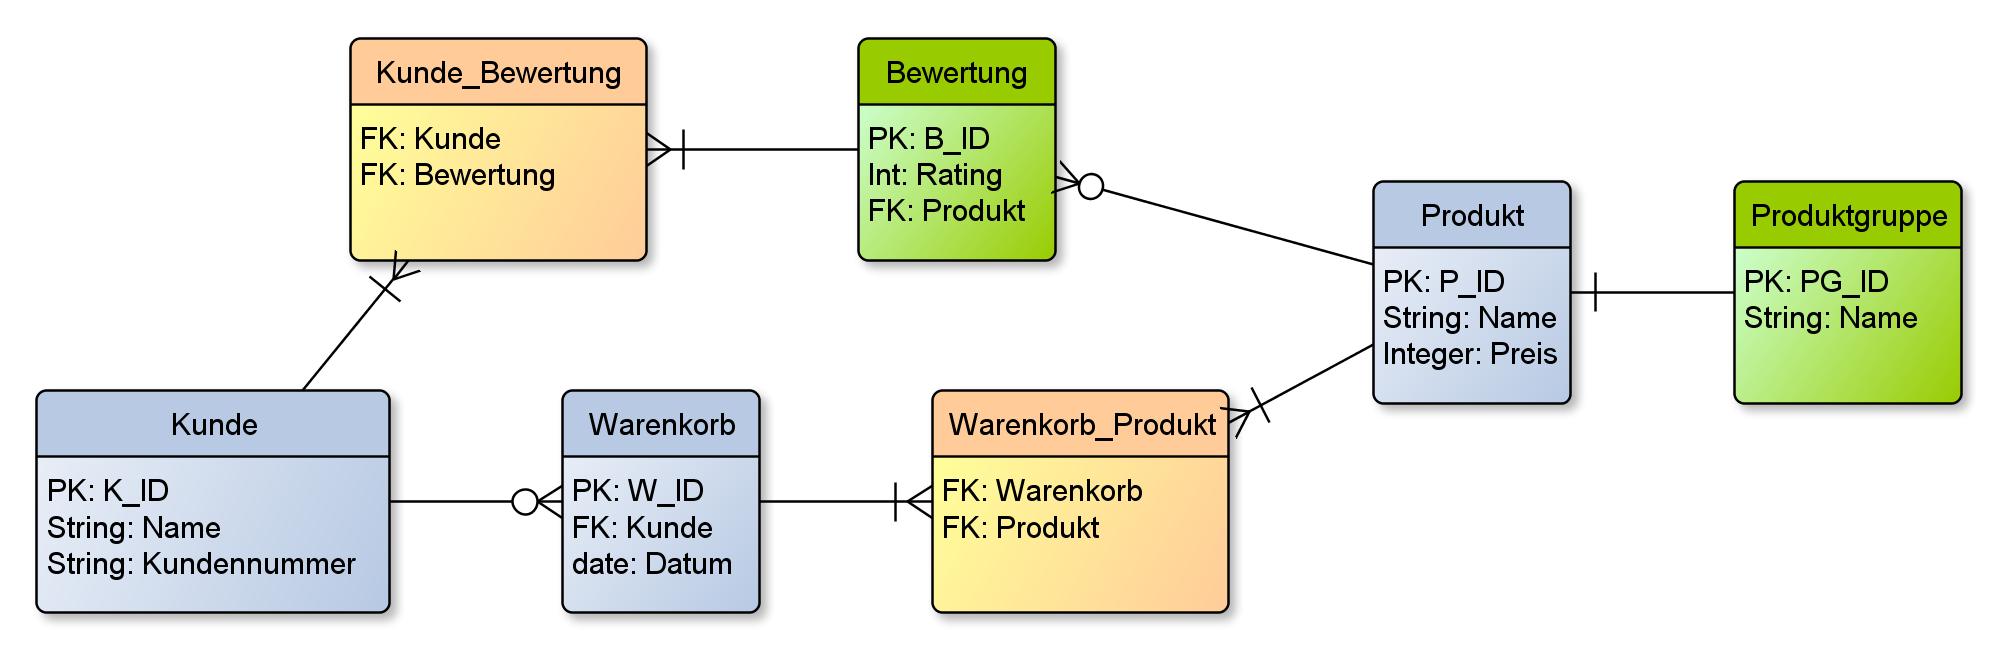
\includegraphics[width=1.0\textwidth]{Steff/ADBC-ERD.png}
	\caption{Orginal-ERD}
	\label{fig:ADBC_ERD}
\end{figure}

Das ERD beschreibt die Architektur unserer Datenbank. Die urspr�ngliche Planung sah vor, dass die Datenbank bei ausreichender Zeit noch erweitert werden konnte um mehr Anwendungsf�lle simulieren zu k�nnen. In diesem Fall w�ren die Tabellen die gr�n markiert sind, sowie die angrenzenden Verbindungsverbindungstabellen (rot markiert) zus�tzlich erstellt worden.
Die Tabellen mit der h�chsten Priorit�t waren aber Kunde, Warenkorb und Produkt. Dadurch wurde das Datenmodell, welches letzten Endes erstellt wurde, �u�erst kompakt.\\
Anm.: Grafik wird noch generiert\\
\subsection{Datenbankabfragen}
\begin{figure}[h]
	\centering
		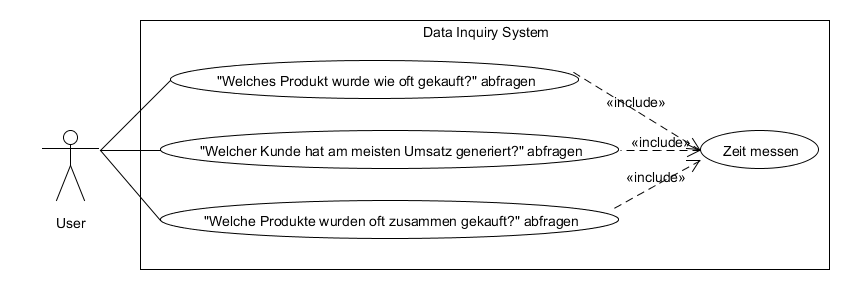
\includegraphics[width=1.0\textwidth]{Steff/UC.png}
	\caption{Datenbankabfragen}
	\label{fig:AbfragenUC}
\end{figure}
Da unser Projekt einen Webshop imitieren sollte, haben wir unsere Anwendungsf�lle so gew�hlt, wie sie auch in der Realit�t gefunden werden k�nnen. Sie k�nnten unter anderem Managern bei der Auswertung ihrer Gesch�fte dienen. Das gesamte Spektrum an m�glichen Abfragen abzudecken, h�tte jedoch den Zeitrahmen extrem gesprengt. Deshalb wurde sich f�r die folgenden vier Abfragen entschieden:
\begin{itemize}
	\item Welches Produkt wurde wie oft gekauft?
	\item Wieviel Umsatz wurde von wem in einem bestimmtem Zeitraum generiert?
	\item Wie viele Kunden haben an einem bestimmten Zeitpunkt bestellt?
	\item Wer hat wieviel an den gegebenen neun Tagen umgesetzt?
\end{itemize}
Diese Abfragen haben unterschiedliche Komplexit�ten. So m�ssen bei der zweiten Abfrage s�mtliche Tabellen einbezogen werden, w�hrend bei der ersten Abfrage nur zwei Tabellen involviert sind.
Auf diese Weise soll ein m�glichst breites Spektrum an Abfragen getestet werden, um sicher zu stellen, dass die Versuche so aussagekr�ftig wie m�glich werden.